\chapter{Gestion du projet}

\section{Répartition des tâches}
Dans un premier temps, nous avons segmenté l’implémentation de notre projet en travaillant sur les deux fonctionnalités principales: la récupération des événements, et la recherche dans l’annuaire. \\
Etant donné que pour chacune de ces deux tâches, il fallait s’occuper séparément de la partie concernant l’Université de Bordeaux 1 et de celle concernant le LaBRI, quatre tâches distinctes étaient à notre disposition ce qui nous a permis de répartir aisément le travail entre les membres de l’équipe. Le fait que certaines de ces tâches étaient plus simples à implémenter que d’autres, nous a permis d’avoir beaucoup d’interactions entre développeurs et donc beaucoup d’entraide.\\\\

Une fois que nous avons constaté que l’implémentation des fonctionnalités principales évoluait vite et qu’elle était quasiment finalisée, nous avons orienté deux membres de l’équipe pour s’intéresser aux fonctionnalités secondaires de notre application: l’accès aux emplois du temps, et le plan du campus. Là aussi avaient lieu beaucoup d'interactions dans l’équipe afin de pouvoir disposer de l’avis de plusieurs personnes lors de l’implémentation de certaines fonctionnalités.\\
Une fois les tâches secondaires finies, l’application était à un stade très avancé, tous les besoins fonctionnels  étaient achevés, il ne manquait alors plus que quelques touches de finalisation à apporter au sein des fonctionnalités principales. L’ensemble des membres de l’équipe ont alors pu contribuer à la mise au point finale.\\
Durant la phase finale de test, la répartition des tests à effectuer a été faite en fonction des tâches que chacun des membres a effectuées.\\
Le diagramme de Gantt ci-dessous présente une première estimation de la répartition des tâches sur le déroulement du projet. Chaque ligne représente une tâche à effectuer, une estimation de sa durée, et son attribution au sein de l'équipe de développement. \\


\begin{figure}[h]
  \center
  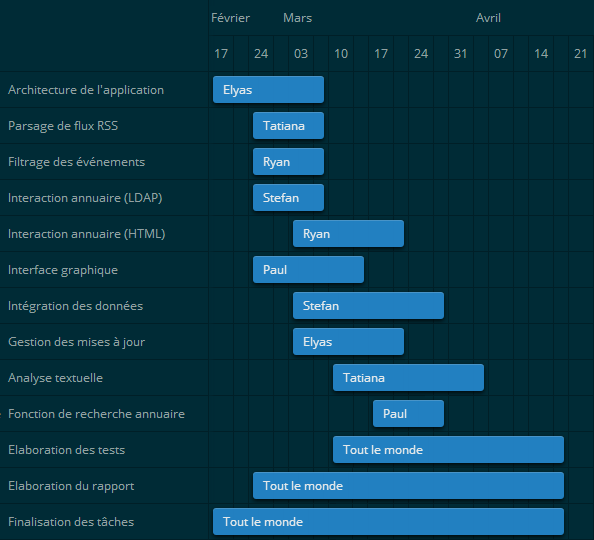
\includegraphics[width=0.8\textwidth]{resources/gantt.png}
  \caption{Diagramme de Gantt des répartitions des tâches.}
\end{figure}


\section{Outils de développement}
Dès le début de notre projet, nous avons décidé d’utiliser \emph{git} qui nous a paru être une solution plus complète comparée à \emph{svn}. Au fur et à mesure que nous pensions à une tâche à effectuer, ou que nous détections un bug à corriger, nous avons ajouté une \emph{issue} (problème ou tâche à effectuer) à notre projet sur GitHub. L’issue tracker de GitHub est très pratique, il permet de trier les issues par catégories, de les assigner à des membres du projet, ou encore d’ajouter des commentaires. De plus il suffit de préciser le numéro de l’issue que l’on corrige lors d’un commit pour fermer cette tâche automatiquement. Git offre également la possibilité de créer des branches qui permettent d’implémenter des fonctionnalités séparément, puis de fusionner les branches une fois terminée.

\section{Tests Unitaires}
Afin de s'assurer que notre code soit robuste, nous avons effectué des tests unitaires, afin de s'assurer que toutes les parties de notre code fonctionnent correctement. Nous avons déterminé que les unités les plus petites de notre projet sont les classes ; les tests unitaires portent donc sur ces éléments. Les classes les plus importantes de l’application sont les \emph{Activity}, car elles s’occupent du fonctionnement de chaque partie de l’application (notamment les événements et l'annuaire). Il a donc fallu tester ces classes en priorité.\\
Pour cela, nous avons utilisé Robotium, un outil open-source pour l'élaboration de tests sous Android. Il permet notamment de simuler toutes sortes d'intéractions avec l'interface graphique (clicks, touches longues, glissements et autres mouvements). Ainsi, nous avons pu implémenter des tests sur l'interface, réalisant quelques uns de nos tests d'utilisation.\\
Cet outil permet également de tester la couverture de code des applications Android, mais malheureusement ne supporte pas correctement les projets de tests ayant des dépendances externes, ce qui nous a donc empêché d'analyser la couverture du code de notre projet.\\

L'application étant dépendante d'un parsage de données téléchargées dont nous ne contrôlons pas le contenu, nous devons être sûrs que les parseurs fonctionnent le mieux possible. Nous avons donc effectué des tests à la fois avec du contenu contrôlé (que nous avons écrit et qui correspond aux formats des données que nous avons pu identifier sur les flux et les pages téléchargées), et avec du contenu réel, afin de s'assurer du bon fonctionnement de nos parseurs.
Il était également important de tester la classe \emph{TimeExtractor}, afin d'être sûr que nous avions les dates correctes au cours du parsage et que l'ajout d'un événement important dans l'agenda du smartphone ne produirait pas une horaire décalée. Cela évitera qu'un utilisateur soit en retard à un événement à cause de notre application.
